\chapter{General Poisson Point Processes}
\textbf{Reference} Lectures on the Poisson Process (Penrose), Poisson Processes (Kingman)

\section{Introduction}
\textbf{Question} How can we represent points on $\mathbb{R}_+$ mathematically?
\begin{enumerate}
	\item A set of points $\mathcal{S}=\{S_1, S_2, \ldots \}$ \label{q:3}
	\item 'Time point of view', ie $T_1,T_2, \ldots $ where $T_i$ = time between the $(i-1) $'th and $i $'th point. \label{q:1}
	\item Cadlag formulation with values in $ \mathbb{N}$. $N_t=$ number of points in $[0,t]$. \label{q:2}
	\item Measure $N: \mathcal{B}(\mathbb{R}_+) \to \mathbb{N}$ with $N(A)=$ number of points in $A$. \label{q:4}
\end{enumerate}
\textbf{Goal} Define $\Omega \to $'set of points'. For a general state space $\mathbb{R}^2, [0,1]^2,$ a manifold, etc. 
\ref{q:1} and \ref{q:2} are specific to $\mathbb{R}_+$, so they do not generalize. \ref{q:3} is not very easy to describe. \ref{q:4} is actually nice, so we will  use this point of view.

\textbf{Framework} $(E,d)$ a Polish space (separable, complete, metric space). $\mathcal{E}$ Borel $\sigma$-algebra. $\mu: \sigma$ finite measure on $(E, \mathcal{E})$, i.e. there exist $B_i \uparrow E$ such that $\mu(B_i)<\infty$ where $B_i \uparrow E$ if and only if $B_1 \subset B_2 \subset \ldots$ with $\bigcup_{i\geq 1}B_i=E$.

\begin{ex}[] Of such spaces: 
\begin{enumerate}
	\item $E=\{0\},\ \mu = \delta_0$
	\item $E=\mathbb{R}_+,\ \mu = \lambda \mathcal{L}$
	\item $E=\mathbb{R}^2,\ \mu(dx)=\frac{1}{\pi} e^{- |x|^2}dx$ 'Gaussian'
\end{enumerate}
\end{ex}

\textbf{Idea} We wish to define a point process on $(E, \mathcal{E})$ where the 'number of points around $x$ ' $\approx \mu(dx)$ on $\mathbb{R}_+$. 

\section{Point Processes}
\textbf{Notation} 
\begin{align}
	\mathcal{N}=\{\sigma-\textrm{finite measures: } \forall B \in \mathcal{E}: \nu(B) \in \mathbb{N} \cup \{+\infty\}\}.
\end{align}

\noindent
\textbf{Measure Structure} Let $\mathcal{B}(\mathcal{N})$ be the $\sigma$-algebra generated by the sets $\{\nu \in \mathcal{N}: \nu(B)=k\}=\mathcal{N}_k$ for $B \subset E$ measurable and $k \in \mathbb{N}$. $\to (\mathcal{N}, \mathcal{B}(\mathcal{N}))$ measured space.

\begin{prop}[Representation as Dirac Sum]
	Let $\mathcal{N}_{<\infty}=\{\eta \in \mathcal{N}: \eta(E)<\infty \}$, there exists measurable maps $\tau: \mathcal{N}_{< \infty} \to \mathbb{N}$ and $ X_i: \mathcal{N}_{< \infty} \to E$ such that 
	\begin{align}
		\forall \eta \in \mathcal{N}_{<\infty}\quad \eta = \sum_{i=0}^{\tau(\eta)} \delta_{X_i(\eta)}.
	\end{align}
\end{prop}
\begin{rmk}[]
	Thus $\eta$ corresponds to a collection of points $\{X_1, \ldots ,X_{\tau}\}$.
\end{rmk}
\begin{proof}
	Fix $ \mathcal{Y}=\{y_1,y_2,\ldots\}$ countable and dense in $E$. (WLOG we can assume that $E$ is infinite). We have $\mathcal{N}= \bigcup_{k=0}^{\infty}\mathcal{N}_{k}$ (disjoint) where $\mathcal{N}_{k}=\{ \eta:\ \eta(E)=k\}$. We prove by induction on $k\geq 0$ that for every $k\geq 0$ there exist $Z_1,\ldots ,Z_k:\ \mathcal{N}_{k} \to E$ measurable such that 
	\begin{align}
		\forall \eta \in \mathcal{N}_{k} \quad \eta = \sum_{i=1}^{k} \delta_{Z_i}.
	\end{align}
	For $k=0$ there is nothing to prove. Let $k\geq 0$ and assume that the property holds. Let $\eta \in \mathcal{N}$ such that $\eta(E) = k+1$. We will construct by induction $Y_1(\eta), Y_2(\eta),\ldots \in \mathcal{Y}$ such that for all $n$ $Y_n$ is measurable (as a mapping from $\mathcal{N}_{k+1} \to E$ ) and such that for all $n$ $\eta( \bigcup_{m\leq n}B(Y_m,\frac{1}{m})) \geq 1$.	

\noindent \textbf{Construction of $Y_1$}
We have $1\leq \eta(E) \leq \sum_{i> 0}^{} \eta ( B(y_i,1))$, because $E=\bigcup_{i> 0}B(y_i,1)$. Define $i_{1}= \min\{i:\ \eta(B(y_i,1))\geq 1$ \} and set $Y_1(\eta) = y_i$. $Y_1$ is measurable because 
\begin{align}
	\{ Y_1(\eta ) =y_j\} = \bigcap _{i<j}\{ \eta(B(y_i, 1))=0 \} \cap \{ \eta (B(y_i, 1))=1\}.
\end{align}

\noindent \textbf{Construction of $Y_n$} 
Assume that $Y_1,\ldots ,Y_{n-1}$ have already been constructed. Let $C=\bigcap_{1\leq m \leq n-1}B(Y_m (\eta), \frac{1}{m})$. We have 
\begin{align}
	1 \leq \eta(C) \leq \sum_{i> 0}^{} \eta \left( C \cap B\left(y_i, \frac{1}{n}\right)\right).
\end{align}
Define $Y_n(\eta) = y_{i_{n}}$ where $i_{n}=\min\{ i:\ \eta(C \cap B(y_i, \frac{1}{n})) \geq 1\}$. As above, $Y_n$ is measurable.

The sequence $(Y_n)_{n\geq 0}$ constructed above is a Cauchy sequence (indeed for every $n\geq m$ $B(Y_n, \frac{1}{n}) cap B(Y_m, \frac{1}{m}) \neq \emptyset$, hence by the triangle inequality $d(Y_n, Y_m) \leq \frac{2}{m}$). Define $Z_{k+1}(\eta) = \lim_{n\to \infty }Y_{n}(\eta)$ ($Z_{k_1}$ is measurable as a simple limit of measurable functions). Furthermore $\{Z_{k+1}(\eta)\} = \bigcap_{n> 0}B(Y_n, \frac{2}{n})$ and therefore $\eta(\{Z_{k+1}(\eta) \}) \geq 1$. 

Define $\eta' = \eta - \delta_{Z_{k+1}(\eta)}$ ($\eta'$ is measurable in $\eta$), {\color{blue}note that} $\eta'(E) =k$. By induction, there exist $Z_{1}'(\eta'),\ldots, Z_{k}'(\eta')$ such that $\eta' = \delta_{Z_1'}+\ldots + \delta_{Z_k'}$, we obtain
\begin{align}
	\eta = \sum_{i=1}^{k+1} \delta_{Z_i(\eta)}.
\end{align}
\end{proof}

\begin{defn}
	Let $(\Omega, \mathcal{F}, \mathbb{P}_{}) $ be a probability space. A \emph{point process} on $(E, \mathcal{E})$ is a random variable $N$ defined on $\Omega $ with values in $\mathcal{N}$.
\end{defn}

'$N$ is a random measure.'

This means $N: \Omega \to \mathcal{N};\ \omega \mapsto N_{\omega } $ is measurable. For any fixed $B \subset E$ we can consider $N(B): \Omega \to \mathbb{N}\cup \{+\infty\};\ \omega \mapsto N_{\omega }(B)$ and one can directly check that $N(B)$ is a random variable. 
'$N(B)=$ number of points in B'.

\begin{ex}[] Point Processes:
\begin{itemize}
	\item $N=0$ a.s.  $\to$ empty set
	\item $E=[0,1], X$ random variable on  $[0,1]$.  $N=\delta_X$ is a point process.
	\item $X_1, \ldots X_n$ i.i.d. random variable on $[0,1]$,  $N=\delta_{X_1}+ \ldots +\delta_{X_n}$ is a point process.
\end{itemize}
\end{ex}

\section{Poisson Point Processes}
\textbf{Setup} $(E, \mathcal{E})$ Polish, $\mu$ fixed $\sigma$-finite measure (think of $\lambda \mathcal{L}$ ), $\mathcal{N}=\{\sigma$ finite counting measure$\}$, $(\Omega, \mathcal{F}, \mathbb{P} )$ a probability space.

\begin{defn}
	A Poisson process with intensity $\mu$ on $(E, \mathcal{E})$ (ppp$(\mu)$) is a point process such that
 \begin{enumerate}
	 \item For all $B_1 \ldots B_k \subset E$ measurable and disjoint, $N(B_1), \ldots ,N(B_k)$ are independent.
	 \item For all $B \subset E$ measurable, $N(B)$ has law Pois$(\mu(B))$.
\end{enumerate}
\end{defn}
\begin{rmk}[]
	For all $B \subset E$ measurable
	\begin{align}
		\mathbb{E}_{} \left[ N(B) \right] = \mu(B),
	\end{align}
	'on average, there are $\mu (B)$ points in $B$.
\end{rmk}

\begin{theorem}[Representation as a proper process]
	Let $N$ be a ppp$(\mu)$ on $(E, \mathcal{E})$. There exists some random variable $\tau \in \mathbb{N}\cup \{\infty\}$ and $X_n \in E$, $n> 0$ defined on $\Omega $ such that
	\begin{align}
		N = \sum_{n=1}^{\tau} \delta_{X_n}.
	\end{align}
\end{theorem}

\begin{proof}
	Let $B_i \uparrow E$ such that $\mu (B_n) < \infty $. Let $A_j = B_i \setminus B_{i-1}$, $n\geq 0$ ($A_n$ are disjoint and their union is  $E$).  The process $N_i := N(\ \cdot \ \cap A_i)$ takes values in $\mathcal{N}_{<\infty }$. Hence the proposition in the previous section ensures that there exist some random variables $\tau^{(i)}, Z_1^{(i)}, \ldots, Z_{\tau}^{()}$ such that
	\begin{align}
		N_i = \sum_{j=1}^{\tau^{(i)}} \delta_{Z_{j}^{(i)}} \textrm{ a.s.}
	\end{align}
Use that $N=\sum_{i=1}^{\infty } N_i$, and a reordering of the terms in the sums, we obtain the desired result.	
\end{proof}


\textbf{Question} Does there always exist a ppp$(\mu)$ on $E$?
\section{Existence and Uniqueness}
\subsubsection{Spaces with finite measure}
\begin{prop}[]
	Let $Z$, $(X_i)_{i\geq 1}$ be independent random variables. 
	\begin{align}
		Z \sim \textrm{Pois}(\mu(E)), \quad X_i \sim \frac{\mu(\ \cdot \ )}{\mu (E)}.	
	\end{align}
	Then $N= \sum_{i=1}^{Z} \delta_{X_i} $ is a ppp$(\mu)$ on $E$.
\end{prop}
{\color{blue}
TODO: example}

\begin{proof}
	Let $B_1, \ldots B_{k-1} \subset E$ be disjoint and measurable. Set $B_k = E \setminus \left( \bigcap_{i=1}^{k}B_i \right)$. Let $n=n_1+ \ldots + n_k$. Define $Y_i = \sum_{j=1}^{n} \mathbbm{1}_{X_j \in B_i}$. Observe that $(Y_1,\ldots , Y_k)$ has a multinomial$(\frac{\mu (B_1)}{\mu(E)},\ldots , \frac{\mu (B_k)}{\mu (E)})$ independent of $Z$.

We have 
\begin{align}
	\mathbb{P}_{} \left[ N(B_1)=n_1, \ldots , N(B_k)=n_k \right] &=\mathbb{P}_{} \left[ Z=n, Y_1=n_1,\ldots ,Y_k=n_k \right] \\
								     &= \frac{\mu (E)^{n}}{n!}e^{-\mu (E)} \cdot \frac{n!}{n_1! \cdots n_k!} \left( \frac{\mu (B_1)}{\mu (E)}\right)^{n_1}\cdots  \left( \frac{\mu (B_k)}{\mu (E)}\right)^{n_k} \\
								     &= \prod_{i=1}^{k}\frac{\mu (B_i)^{n_i}}{n_i!}e^{-\mu (B_i)}.
\end{align}
By summing over all $n_k$, we get 
\begin{align}
	\mathbb{P}_{} \left[ N(B_1)=n_1,\ldots , N(B_{k-1})=n_{k-1} \right] = \prod_{i=1}^{k-1}\frac{\mu (B_i)^{n_i}}{n_i!}e^{-\mu (B_i)}.
\end{align}
Hence $N(B_1),\ldots , N(B_{k-1})$ are independent Pois$(\mu (B_i))$ random variables.
\end{proof}


\subsubsection{Superposition}
\begin{lemma}[]
	Let $\lambda = \sum_{i=1}^{\infty} \lambda_i,\ \lambda_i\geq 0$. $(X_i)_{i> 0}$ independent random variables with Pois$(\lambda_i)$ distribution, then $X = \sum_{i=1}^{\infty} X_i$ is a Pois$(\lambda)$ random variable.
\end{lemma}
\textbf{Convention} $X \sim \textrm{Pois}(\infty)$ if and only if $X=\infty $ a.s.
\begin{proof}
	Exercise.
\end{proof}


\begin{theorem}[]
	Let $N_i, i\geq 1$ be a sequence of independent ppp$(\mu_i)$ where $\mu_i$ and $\mu = \sum_{i=1}^{\infty} \mu_i$ are $\sigma$-finite measures. Then $N= \sum_{i=1}^{\infty} N_i$ is a ppp$(\mu )$.
\end{theorem}
\begin{proof}
	We first check that $N$ is a point process. Let $B_n \uparrow E$ be such that $\mu (B_n)<\infty $. For all $n$ $N(B_n)=\sum_{i=1}^{\infty } N_i(B_n)$. Since $\mu(B_n)<\infty $, $N(B_n)<\infty $ a.s. Hence N is a $\sigma $-finite measure almost surely. Furthermore for every $B\subset E$ measurable $N(B) = \sum_{i}^{} N_i(B)$ is measurable, hence $N$ is measurable.

	For $B\subset E$ measurable, 
	\begin{align}
		N(B) = \sum_{i}^{} N_i(B){\color{blue} \stackrel{\textrm{(d)}}{=} \sum_{i}^{} \textrm{Pois}(\mu_i(B_n))}.
	\end{align}
	By the lemma, $N(B)$ is a Pois$(\mu (B))$ random variable. Finally for $B_1,\ldots , B_k \subset E$ measurable and disjoint $\left( N_i(B_j)\right)_{i \in \mathbb{N},1\leq j \leq k}$ are independent random variables. Therefore $N(B_i)=\sum_{i}^{} N_i(B_1) , \ldots , N(B_k) =\sum_{i}^{} N_i(B_k)$ are independent by grouping.
\end{proof}


\begin{cor}[]
Assume that $\mu$ is a $\sigma$-finite measure on $(E, \mathcal{E})$, then there exists a ppp$(\mu)$ on $E$.
\end{cor}
\begin{proof}
	$\mu = \sum_{i=1}^{\infty } \mu _i$ where $\mu _i(E) < \infty $. Let $(N_i)$ be independent Poisson processes, where $N_i$ is a ppp$(\mu _i)$. Define $N= \sum_{i=1}^{\infty } N_i$, by superposition, $N$ is a ppp$(\mu )$.
\end{proof}

{\color{blue}
TODO: Example}

\subsubsection{Uniqueness}
Let $N$ be a ppp$(\mu )$ on $E$, its law $P_N$ is a probability measure on $ \mathcal{N}$.

\begin{prop}[]
	Let $N, N'$ be two ppp$(\mu )$ on $(E, \mathcal{E})$ then $P_N = P_{N'}$.
\end{prop}
\begin{rmk}[]
	$P_N = P_{N'}$ if and only if for all $A \subset \mathcal{N}$ measurable $P_N(A) = P_{N'}(A)$ if and only if for all $A \subset \mathcal{N}$ measurable $\mathbb{P}_{} \left[ N \in A  \right]  = \mathbb{P}_{} \left[ N' \in A \right] $. 
\end{rmk}

\begin{proof}
Let $B_1,B_2 \subset E$ measurable, $n_1,n_2\geq 0$. Define $C_1 = B_1 \setminus B_2$, $C_2 = B_1 \cap B_2$, and $C_3= B_2 \setminus B_1$. 

\begin{figure}
	\centering
	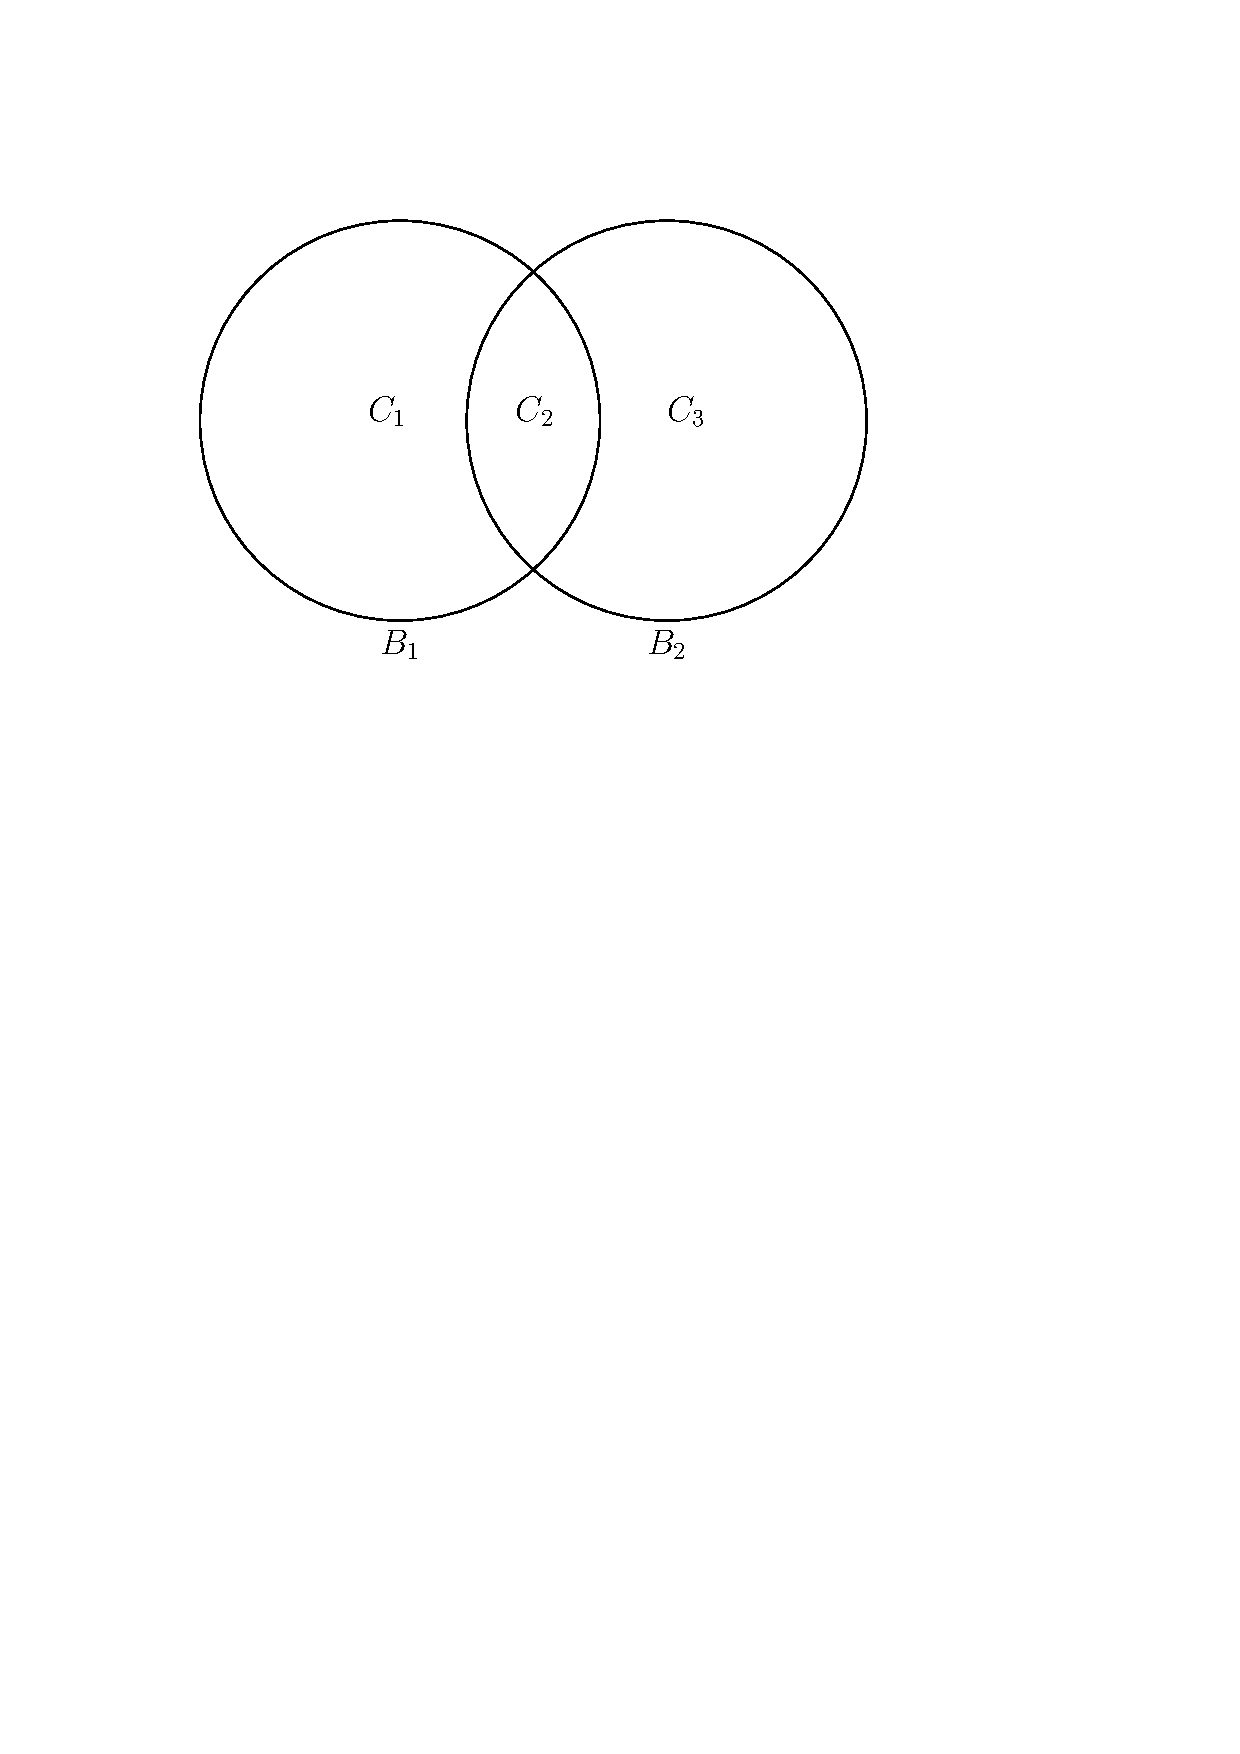
\includegraphics[width=0.5\textwidth]{figures/intersection.pdf}
\end{figure}


\begin{align}
	\mathbb{P}_{} \left[ N(B_1)=n_1, N(B_2)=n_2 \right] &= \sum_{\substack{m_1+m_2 = n_1\\ m_2+m_3 = n_2}}^{} \mathbb{P}_{} \left[ N(C_1) = n_1, N(C_2)=m_2, N(C_3)=m_3 \right] \\ 
							    &= \sum_{\substack{m_1+m_2 = n_1\\ m_2+m_3 = n_2}}^{} \mathbb{P}_{} \left[ N'(C_1)=m_1, N'(C_2)m_2,N'(C_3)=m_3 \right] \\
							    &= \mathbb{P}_{} \left[ N'(B_1)=n_1, N'(B_2)=n_2 \right] 
\end{align}
Where the second equality holds as the $C_i$ are disjoint. Equivalently, for all $B_1,\ldots , B_k \subset E$ measurable
\begin{align}
	\mathbb{P}_{} \left[ N(B_1)=n_1,\ldots , N(B_k)=n_k \right] = \mathbb{P}_{} \left[ N'(B_1)=n_1, \ldots, N'(B_k)=n_k \right]. 
\end{align}
Therefore $P_N(A) \stackrel{(*)}{=} P_{N'}(A)$ for every set of the form $A=\{\eta: \ (\eta(B_1),\ldots ,\eta(B_k) ) \in K\}$ for $B_1,\ldots ,B_k \subset E$ measurable and $K \subset \mathbb{N}^{k}$. Such sets for a $\pi $-system and generate $\mathcal{B}(\mathcal{N})$. Hence, by Dynkin's lemma, $(*)$ holds for every measurable set $A \subset \mathcal{N}$ measurable.  
\end{proof}

\section{Laplace Functional}
\begin{lemma}[]
Let $X$ be a Pois$(\lambda )$ random variable, for $\lambda > 0$, then for all $u\geq 0$ 
\begin{align}
\mathbb{E}_{} \left[ e^{-u X} \right] = \exp( - \lambda (1 - e^{-u})).
\end{align}
\end{lemma}
\begin{proof}
	\begin{align}
		\mathbb{E}_{} \left[ e^{-u X} \right] = \sum_{k}^{} \frac{\lambda^{k}}{k!}e^{-\lambda }e^{-ku} = e^{-\lambda }\exp(\lambda e^{-u})
	\end{align}
\end{proof}

\begin{defn}
	Let $N$ be a point process on $(E, \mathcal{E})$, for every $u:E\to \mathbb{R}_+$ measurable define 
	\begin{align}
		\boxed{		L_N(u) = \mathbb{E}_{} \left[ \exp(- \int u(x) N(dx) \right]. }
	\end{align}
\end{defn}

\begin{rmk}[]
	$L_N(u)$ is well defined. Indeed $\int_E u(x) N(dx) = \int_E u dN$ is a well defined random variable.
\end{rmk}

We can interpret $\int_{}^{} u(x)N(dx)$ as $\sum_{x \textrm{ 'points of N'}}^{} u(x)$ with multiplicities counted.

\begin{theorem}[Characterization via Laplace Functional]
	Let $\mu$ be a $\sigma$-finite measure on $(E, \mathcal{E})$. Let $N$ be a point process on $E$. The following are equivalent
\begin{enumerate}
	\item $N$ is a ppp$(\mu)$, 
	\item For all $u:E \to \mathbb{R}_+$ measurable 
		\begin{align}
			L_N(u) = \exp\left(- \int_E 1- e^{-u(x)} \mu (dx)\right).
		\end{align}
\end{enumerate}
\end{theorem}
\begin{proof}
	'$\Longrightarrow$'
	Let $u=\sum_{i=1}^{k} u_i \mathbbm{1}_{B_i} $ for $B_1,\ldots , B_k$ disjoint, $u_i\geq 0$.
	\begin{align}
		L_{N}(u) &= \mathbb{E}_{} \left[ \exp \left( - \sum_{i=1}^{k} u_iN(B_i) \right) \right]  \stackrel{\textrm{(indep.)}}{=} \prod_{i=1}^{k}\mathbb{E}_{} \left[ e^{u_iN(B_i)} \right] \\
			 &=\prod_{i=1}^{k} \exp\left( -\mu (B_i) (1-e^{-u_i}) \right) = \exp \left( - \int_{E}^{} 1-e^{-u(x)}\mu (dx) \right).
	\end{align}
	For general $u\geq 0$, consider $(u_n)$ of the form above such that $u_n \uparrow u$. For every $n$ 
	\begin{align}
		\underbrace{L_n(u_n)}_{\stackrel{\textrm{(MCT)}}{\to}L_N(u)} = \underbrace{\exp \left( - \int_{E}^{} (1-e^{-u_n(x)})\mu (dx) \right)}_{\to \exp\left( - \int_{E}^{} (1-e^{-u(x)}) \mu (dx)\right)}.
	\end{align}

	'$\Longleftarrow$'
	Let $B_1,\ldots , B_k$ be disjoint. For all $x=(x_1,\ldots ,x_k)$ with $x_i\geq 0$. {\color{blue}If we set $u= \sum_{i=1}^{k} x_i \mathbbm{1}_{B_i} $, we have}
\begin{align}
	\mathbb{E}_{} \left[ e^{-x \cdot (N(B_1),\ldots ,N(B_k))} \right] &= L_{N}(u) \\
									  &= \exp \left( - \int_{E}^{} 1 - e^{-u(x)}\mu (dx) \right) \\
									  &= \prod_{i=1}^{k}\exp \left(-\mu (B_i) (1- e^{-x_i} \right) = \mathbb{E}_{} \left[ e^{-x \cdot Y} \right] ,
\end{align}
where $Y=(Y_1, \ldots , Y_k)$ is a random vector of independent variables. Furthermore $Y_i$ are Pois$(\mu (B_i))$ random variables, since the Laplace transform characterizes the law we have
\begin{align}
	(N(B_1), \ldots ,N(B_k)) \stackrel{\textrm{(law)}}{=} Y.
\end{align}
\end{proof}

\section{Mapping}
$(E, \mathcal{E}), (F, \mathcal{F})$ Polish spaces, $\mu$ a $ \sigma$-finite measure on $E$, and $T:E \to F$ measurable. $T\#\mu $ is the push forward measure of $\mu $ under $T$ ($T\#\mu(B)=\mu(T^{-1}(B))$).

\begin{theorem}[]
	Assume that $T\#\mu$ is $\sigma$-finite. Let $N$ be a ppp$(\mu)$ on $E$, then $T\#N$ is a ppp$(T\#\mu)$ on $F$.
\end{theorem}
\begin{proof}
	Exercise. 
	{\color{blue} // I think we should include this, not including for now so the 1:1 is done//}
\end{proof}

\begin{rmk}
	If $N$ is proper, $N=\sum_{i=1}^{\tau} \delta_{X_i}$, then $T\#N$ is also proper and $T\#N = \sum_{i=1}^{\tau} \delta_{T(X_i)}$.
\end{rmk}

\begin{ex}[]
	$E=\mathbb{R},\ F=\mathbb{Z},\ T:E \to F; x \to \lfloor x \rfloor,\ \mu= \mathcal{L},\ T\#\mu=|\cdot |$.
\end{ex}

\section{Restriction}
\noindent \textbf{Notation} If $\nu $ is a measure on $E$, $C \subset E$ measurable, then we write $\nu _C: \nu(\cdot \cap C)$ 'the measure restricted to $C$'.
\begin{theorem}[Restriction]
	$(E, \mathcal{E})$ general measure spaces, $\mu $ a $\sigma $-finite measure, and $C_1, C_2, \ldots  \subset E$ measurable and disjoint. If $N$ is a  ppp$(\mu)$ on  $E$, then $N_{C_1}, N_{C_2} \ldots $ are independent ppp with respective intensities $\mu_{C_1}, \mu_{C_2}, \ldots $	
\end{theorem}
\begin{proof}
	Without loss of generality, we may assume $E = \bigcap_{i> 0}C_i$. Let {\color{blue}// I use ' instead of $\sim$ as I think the $\sim$ looks worse in latex//} $N_1', N_2', \ldots$ independent ppp with respective intensities $\mu _{c_1}, \mu _{C_2},\ldots$ By superposition $N' = \sum_{i> 0}^{} N_i'$ is a ppp$(\mu )$ (indeed, $\mu = \sum_{i> 0}^{} \mu _i$). For every $B\subset E$ measurable and $j> 0$ 
	\begin{align}
		N'(B \cap C_j) &= \sum_{i> 0}^{} N_i'(B \cap C_j) =
		\begin{cases}
			0 \textrm{ a.s.} & \textrm{if }i \neq j \\
			N_i'(B) \textrm{ a.s.} & \textrm{if } i=j
		\end{cases} \\
			       &= \widetilde{N}_j'(B) \textrm{ a.s.}	
	\end{align}
Hence $N_{C_j}' = N_j'$ a.s. Let $f_1, \ldots, f_k: \mathcal{N} \to \mathbb{R}_+$ measurable. 
\begin{align}
	\mathbb{E}_{} \left[ \prod_{i=1}^{k}f_i(N_{C_i}) \right]  \stackrel{\textrm{(uniqueness)}}{=} 
	\mathbb{E}_{} \left[ \prod_{i=1}^{k}f_i(N_{C_i}') \right] = \mathbb{E}_{} \left[ \prod_{i=1}^{k}f_i(N_i') \right]= \prod_{i=1}^{k}\mathbb{E}_{} \left[ f_i(N_i') \right] . 
\end{align}
Hence $N_{C_1}, \ldots, N_{C_k}$ are independent ppp$(\mu _{C_i})$.
\end{proof}



\section{Simple Processes}
{\color{blue}
\begin{rmk}[]
	For $x \in E,\ \{x\}$ is measurable because $E$ is Polish.
\end{rmk}}

\begin{defn}
	A measure $\eta \in \mathcal{N}$ is said to be \emph{simple} if for every 
	\begin{align}
		\forall x \in E \quad \eta(\{x\}) \leq 1.
	\end{align}
\end{defn}

\begin{prop}[]
	The set $\{\eta: \eta \textrm{ is simple} \}$ is measurable in $ \mathcal{N} $.
\end{prop}
\begin{proof}
	Recall the definition of $\tau:\mathcal{N}_{<\infty } \to \mathbb{N}$ and $X_i: \mathcal{N}_{< \infty } \to E$ in such a way that for all $\eta \in \mathcal{N}_{<\infty }$ $\eta = \sum_{i=1}^{\tau(\eta)} \delta_{X_i(\eta)}$. Therefore
	\begin{align}
		\{\eta \in \mathcal{N}_{< \infty } :\ \eta \textrm{ is simple}\} = \{ \eta \in \mathcal{N}_{< \infty }: \ \forall i<j \leq \tau(\eta) \ X_i(\eta) \neq X_j(\eta) \}
	\end{align}
is measurable.	
\end{proof}

\begin{theorem}[]
	Assume that $\mu $ is a diffuse (for every $x$ $\mu (\{x\}=0$) and $\sigma$ finite measure. Then every ppp$( \mu )$ $N$ is simple a.s.
\end{theorem}
\begin{rmk}[]
	There exist $\tau, X_i$ random variables such that almost surely $N= \sum_{i=1}^{\tau} \delta_{X_i}$ and $X_i$ are disjoint).
\end{rmk}
\begin{proof}
	)Let $B_i \uparrow E$ such that for all $i$ $\mu (B_i)< \infty $. Consider $\mu _i = \mu (\cdot \cap B_i)$ (diffuse). Let $\tau$ be a Pois$(\mu (B_i))$ random variable, $X_1, X_2,\ldots$ i.i.d. where each $X_j$ has law $\frac{\mu _i(\cdot)}{\mu (B_i)}$ {\color{blue}, ie. they are uniform on $B_i$}. As before, the point process $N_i'$ defined by $N_i' = \sum_{j=1}^{\tau} \delta_{X_j}$ is a ppp$(\mu _i)$. 
	\begin{align}
		\mathbb{P}_{} \left[ N_i' \textrm{ not simple} \right]  
		&\stackrel{\phantom{X_j,X_k \textrm{ indep.}}}{\leq} \mathbb{P}_{} \left[ \exists j\neq k:\ X_j = X_k \right]  \leq \sum_{j\neq k}^{} \mathbb{P}_{} \left[ X_j = X_k \right] \\ 
		&\stackrel{X_j,X_k \textrm{ indep.}}{=} \int_{E}^{} \underbrace{\mathbb{P}_{} \left[ X_j=x \right]}_{=0} \frac{\mu _i(dx)}{\mu (B_i)} = 0.
	\end{align}
	Now, let $N$ be any ppp$(\mu )$ on $E$. By restriction $N_{B_i} = N( \cdot \cap B_i)$ is a ppp$(\mu _i)$. By uniqueness 
	\begin{align}
		\mathbb{P}_{} \left[ N_{B_i} \textrm{ simple} \right]  = \mathbb{P}_{} \left[ N_i' \textrm{ simple} \right] =1.
	\end{align}
	Hence $\mathbb{P}_{} \left[ \bigcap_{i> 0} N_{B_i} \textrm{ simple} \right] =1$, which concludes that $N$ is simple a.s.	
\end{proof}

\section{Marking}
\noindent
\textbf{Motivation} Cars on a highway, at time 0 the position of the cars is a ppp$(1)$ on $\mathbb{R}$ (that means on average 1 car per kilometer of highway). We put an observer (Olga) at 0 on $\mathbb{R}$.

Case 1: All of the cars have speed 50km/h, we want to study $X=$ number of cars seen by Olga in 1 hour. What is the law of $X$? $X \sim \textrm{Pois}(50)$.

Case 2: The cars have a random speed $ \sim \mathcal{U}([50,100]) $. What is the law of $X$? It may at first seem complicated, but it is not!

\noindent
\textbf{Framework} $(E, \mathcal{E})$ Polish, $\mu$ $\sigma$-finite. $(F, \mathcal{F}, \nu )$ Polish, probability space ('space of marks').
\begin{defn}
	Let $N=\sum_{i=1}^{\tau} \delta_{X_i}$ be a proper ppp$(\mu)$ on $E$. $(Y_i)_{i> 0}$ i.i.d. random variable with law $\nu $ independent of $N$. The \emph{marked point process} is the point process on $E \times F$ defined by 
	\begin{align}
	\boxed{M=\sum_{i=1}^{\tau} \delta_{(X_i, Y_i)}.}
	\end{align}
\end{defn}

\begin{rmk}[]
	$X_i$ corresponds to the position of the cars in Case 2, and $Y_i$ to their speeds.
\end{rmk}

\begin{theorem}[]
	The marked process is a ppp$(\mu \otimes \nu )$.
\end{theorem}
\begin{proof}
	First we show that M is a pp. For every $B \subset E$ measurable,
	\begin{align}
		M(B) = \sum_{i=1}^{\tau} \underbrace{\mathbbm{1}_{(X_i,Y_i)\in B}}_{\textrm{measurable}}. 
	\end{align}
Let $u:E\times F \to \mathbb{R}_+$ measurable
\begin{align}
	L_M(u) = \sum_{m \in \mathbb{N} \cup \{\infty \}}^{} \underbrace{\mathbb{E}_{} \left[ \mathbbm{1}_{\tau = m} \exp \left(- \sum_{k=1}^{m} u(X_k, Y_k) \right) \right] }_{f(m)}.
\end{align}
For $m<\infty $, we have
\begin{align}
	f(m) &= \int_{F}^{} \ldots \int_{F}^{} \mathbb{E}_{} \left[ \mathbbm{1}_{\tau=m} \exp\left(-\sum_{k=1}^{m} u(X_k, y_k)\right) \right] \nu(dy_1)\ldots \nu(dy_k) \\
	     &= \mathbb{E}_{} \left[ \mathbbm{1}_{\tau = m} \prod_{k=1}^{m}\underbrace{\left( \int_{F}^{} e^{-u(X_k, y_k)}\right)}_{e^{-v(X_k)}} \right] 
\end{align}
where $v(x) = -\log\left(\int_{F}^{} e^{-u(x,y)}\nu(dy) \right) \geq 0$. Hence for all $m < \infty $ $f(m) = \mathbb{E}_{} \left[ \mathbbm{1}_{\tau = m} \exp\left( - \sum_{k=1}^{m} v(x_k)\right) \right] $. Equivalently and using monotone convergence, the equality above also holds for $m=\infty $. Therefore
\begin{align}
	L_m(u) &= \sum_{m \in \mathbb{N}\cup \{\infty \}}^{} \mathbb{E}_{} \left[ \mathbbm{1}_{\tau=m} \exp\left(-\sum_{k=1}^{m} v(X_k) \right) \right] = \mathbb{E}_{} \left[ \exp\left( - \sum_{k=1}^{\tau} v(X_k) \right) \right] \\
	       &= L_{N}(v) = \exp \left( - \int_{E}^{} 1 - e^{-v(x)} \mu (dx) \right) \\
	       &= \exp \left( - \int_{E}^{} \left[ \int_{F}^{} \nu (dy) \ldots \int_{F}^{} e^{-u(x,y)} \nu (dy) \right] \mu (dx) \right) \\
	       &= \exp \left( - \int_{E \times F}^{} 1-e^{-u(x,y)} \nu (dy) \mu (dx) \right).
\end{align}
Hence $M$ is a ppp$(\mu \otimes \nu )$.
\end{proof}


\noindent \textbf{Conclusion} The general ppp we have defined gives us a very general way to talk about a random processes on a large class of spaces (Polish), which fulfill a Markov-like property. This tool will allow us to make much stronger statements in more specific cases.

